\documentclass[8pt, t, aspectratio=169]{beamer}

% ================================
% =  COMPILE WITH XeLaTeX twice  =
% ================================

\usepackage[utf8]{inputenc}
\usepackage[T1]{fontenc}
\usepackage{scrextend}
\usepackage{colortbl}
\usepackage[english]{babel}
\usepackage{xcolor}
\usepackage{framed}
\usepackage{hyperref}
\usepackage{booktabs}
\usepackage{tabularx}
\usepackage{url}
\usepackage{amsmath}
\usepackage{amssymb}
\usepackage{enumitem}

\definecolor{uniSblue}{RGB}{0,65,145}
\definecolor{uniSlightblue}{RGB}{0,190,255}
\colorlet{shadecolor}{uniSlightblue!5!white}
\colorlet{framecolor}{uniSblue!80!white}

\newenvironment{shadedframe}{%
    \def\FrameCommand{\fboxrule=\FrameRule\fboxsep=\FrameSep \fcolorbox{framecolor}{shadecolor}}%
    \MakeFramed {\advance\hsize-\width \FrameRestore}}%
    {\endMakeFramed}
    \setlength\FrameRule{1.5pt}

\mode<presentation>{\usetheme{uniS}}

\pgfdeclareimage[height=.85\paperheight]{background}{bg.jpg}
\pgfdeclareimage[height=1cm]{unilogow}{unilogo.pdf}
\pgfdeclareimage[height=1cm]{ims}{fmi-alg.png}

\newcommand\blfootnote[1]{%
  \begingroup
  \renewcommand\thefootnote{}\footnote{#1}%
  \addtocounter{footnote}{-1}%
  \endgroup
}

\renewcommand*{\thefootnote}{\arabic{footnote}}

\AtBeginSection[]{
  \begin{frame}[plain]
	\sectionpage
  \end{frame}
}

\title{Fachpraktikum \\Algorithmik \\für OSM-Daten}
\author[Lukas Epple]{Lukas Epple}
\institute{Institut für Formale Methoden der Informatik (FMI), Universität Stuttgart}

\begin{document}

\begin{frame}[plain]
  \titlepage
\end{frame}
	    
		
% ===================================================================================
\begin{frame}[plain]{Contents}
\tableofcontents
\end{frame}

\begin{huge}


% ===================================================================================
\section{Introduction}
\begin{frame}{Introduction}
  \vfill
  \begin{itemize}
  \item Implemented Contraction Hierarchies
    \pause
    \item Levels for each node $l: V \rightarrow \mathbb{N}$
    \pause
    \item If a path exists between $u,v \in V$ then it will be found by two upward searches from the $u$ and $v$
    \pause
    \item only using upwards reduces the searchspace

  \end{itemize}
    
  \vfill
\end{frame}

\section{CH-Query}
\begin{frame}{CH-Query}
  \begin{itemize}
  \item given $s, t \in V$, find path from $s$ to $t$ and distance $d(s,t)$
    \pause
  \item perform dijkstra only following edges to nodes with higher levels from $s$ and from $t$
    \pause
  \item $S_s, S_t$ are the settled nodes from the two dijkstras
    \pause
  \item find node $n \in S_s \cap \in S_t$ where $d(s,n) + d(n, t)$ is minimal
  \end{itemize}
\end{frame}

\begin{frame}{CH-Query}
  \centering
  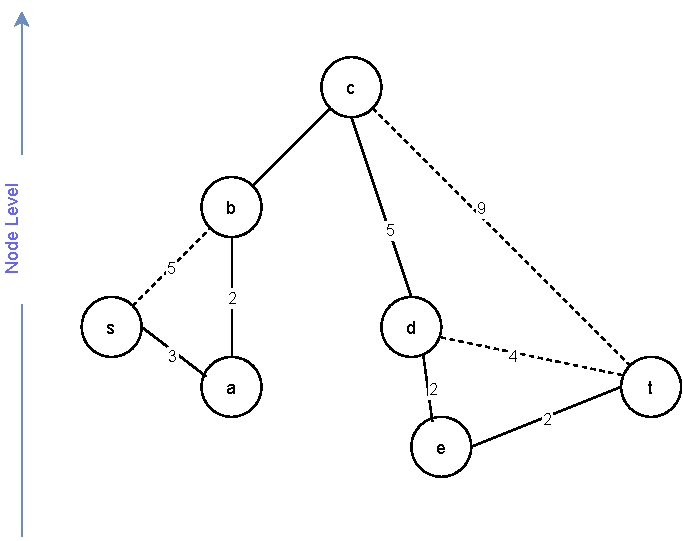
\includegraphics[width=0.5\textwidth]{query1.pdf}
\end{frame}


\begin{frame}{CH-Query}
  \centering
  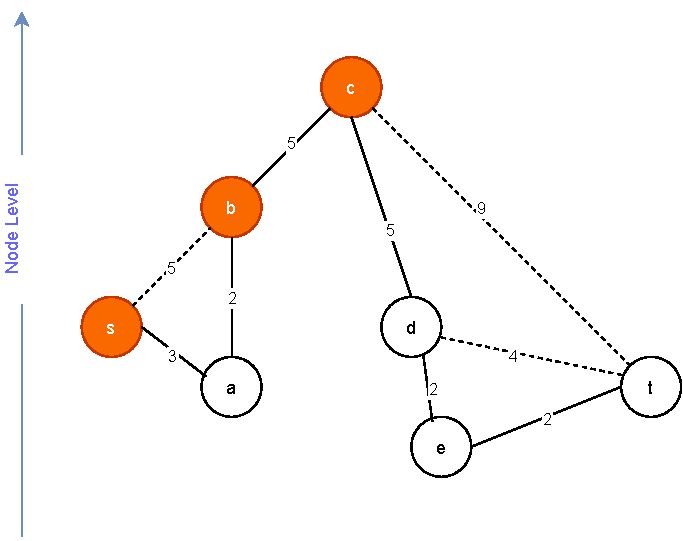
\includegraphics[width=0.5\textwidth]{query2.1.pdf}
\end{frame}

\begin{frame}{CH-Query}
  \centering
  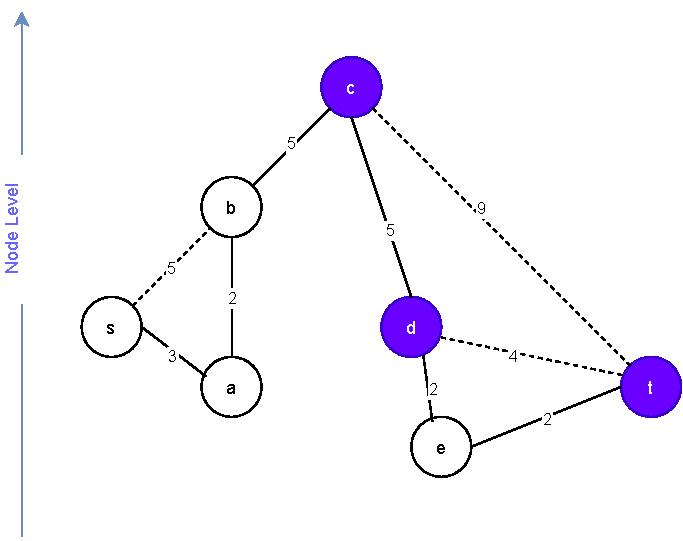
\includegraphics[width=0.5\textwidth]{query2.2.pdf}
\end{frame}

\begin{frame}{CH-Query}
  \begin{minipage}{0.54\textwidth}
    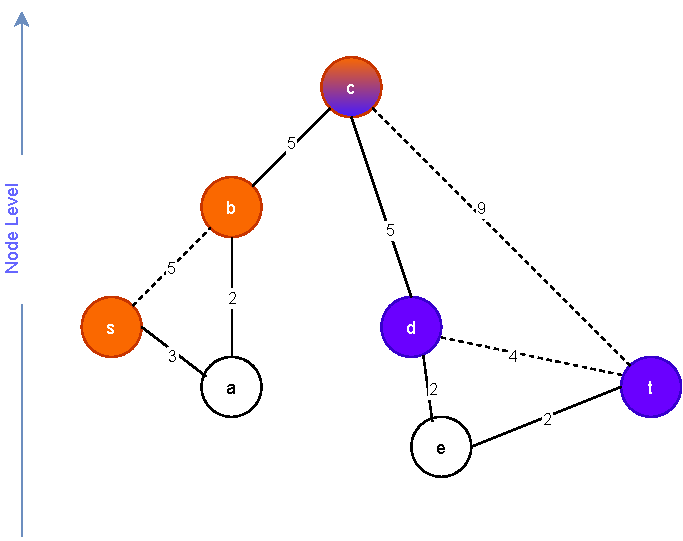
\includegraphics[width=1.0\textwidth]{query2.pdf}
  \end{minipage}
  \pause
  \begin{minipage}{0.44\textwidth}
    \begin{itemize}
    \item $S_s = \{s, b, c\}$
    \item $S_t = \{t, d, c\}$
    \end{itemize}
    \pause
    \Rightarrow $S_s \cap S_t = \{c\}$\\
    \pause
    \Rightarrow $d(s,t)= 19$\\
    \pause
    \Rightarrow recursive unpack the path
  \end{minipage}
\end{frame}
		
% ===================================================================================
\section{Optimizations}
\subsection{Caching Settled Nodes Lists}
\begin{frame}{Caching Settled Nodes Lists}
  \vfill
  \pause
  currently $S_s, S_t$ are cleaned up after a query. \\
  \pause
  \textbf{Idea:} keep $S_s, S_t$ and only clean them up before the next query if needed.

  \pause

  \vfill
  \begin{block}{But\dots}
    This optimization cannot be observed well when benchmarking random $s-t$ queries.
  \end{block}
    
  \vfill

\end{frame}

\subsection{Independent Sets}
\begin{frame}{Independent Sets}
  \vfill
  Currently every node has a different level.\\
  \pause
  \textbf{Idea:} Nodes $x,y \in V$ can have the same level if $xy = e \notin E$
  \vfill

\end{frame}

\begin{frame}{Independent Sets}
  \vfill

  \begin{itemize}
    \pause
  \item Select $U \subseteq V$ such that $\forall x,y \in U: xy \notin E$
    \pause
  \item Contract all nodes $x \in U$
    \pause
  \item Calculate average edge difference ($|shortcuts added| - |edges deleted|$)
    \pause
  \item add contractions where the $edge difference \leq avg edge difference$
  \end{itemize}

  \pause

  \Rightarrow Reduces the preprocessing time

  \vfill

\end{frame}

\subsection{Stall On Demand}
\begin{frame}{Stall On Demand}
  \vfill
  Some Nodes are settled with wrong distances and can never be part of a shortest path.
  \vfill
\end{frame}
\begin{frame}{Stall On Demand}
  \vfill
  \centering
  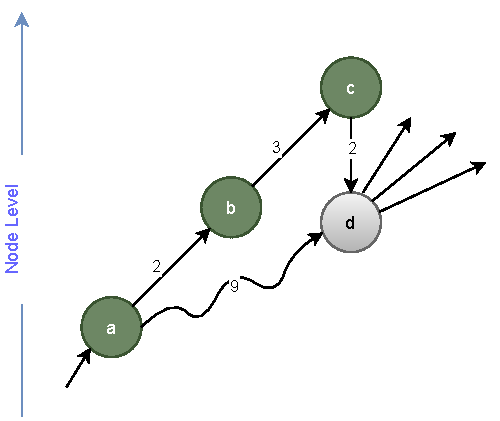
\includegraphics[width=0.5\textwidth]{sod.pdf}
  \vfill
\end{frame}

% ===================================================================================
\section{Benchmarks}
\begin{frame}{Benchmarks}
  \vfill
  The benchmarks compare a normal Dijkstra with an optimized CH-Dijkstra
  \vfill
\end{frame}

\subsection{Heap-Pops}

\begin{frame}{Heap-Pops}
  \vfill
  \centering
  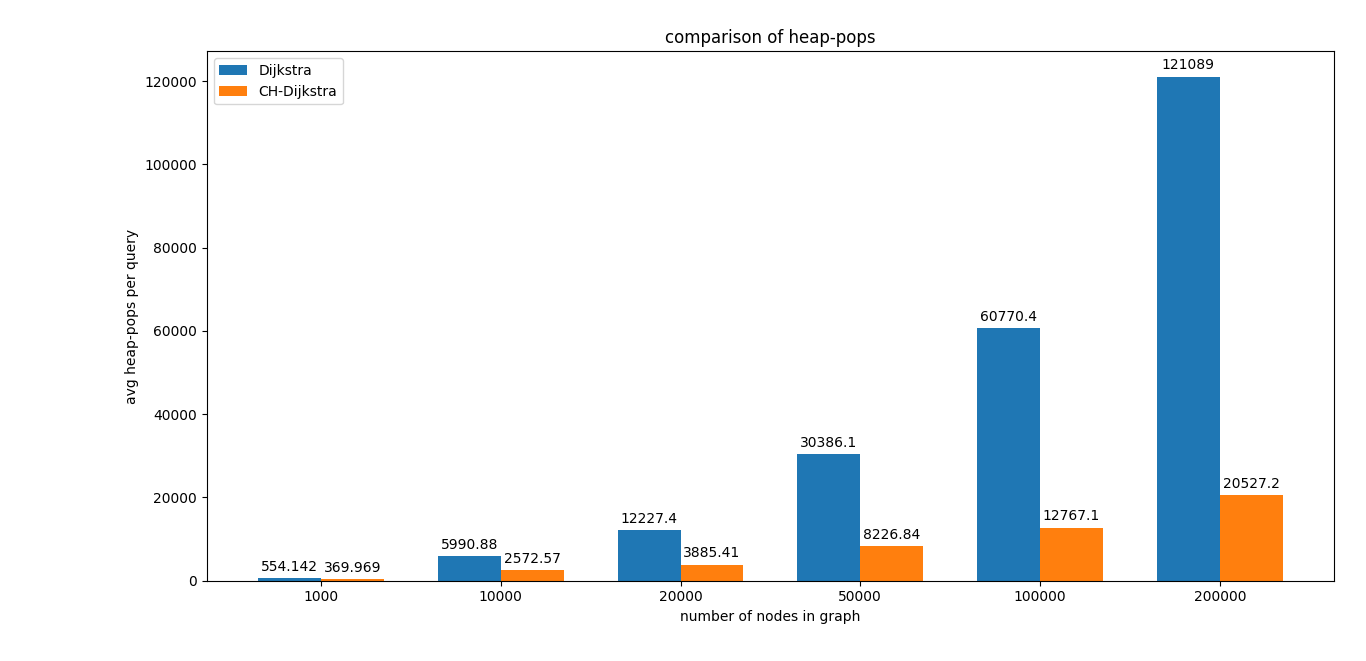
\includegraphics[width=0.9\textwidth]{benchmark-q-pops.png}
  \vfill
\end{frame}

\subsection{Querytime}
\begin{frame}{Querytime}
  \vfill
  \centering
  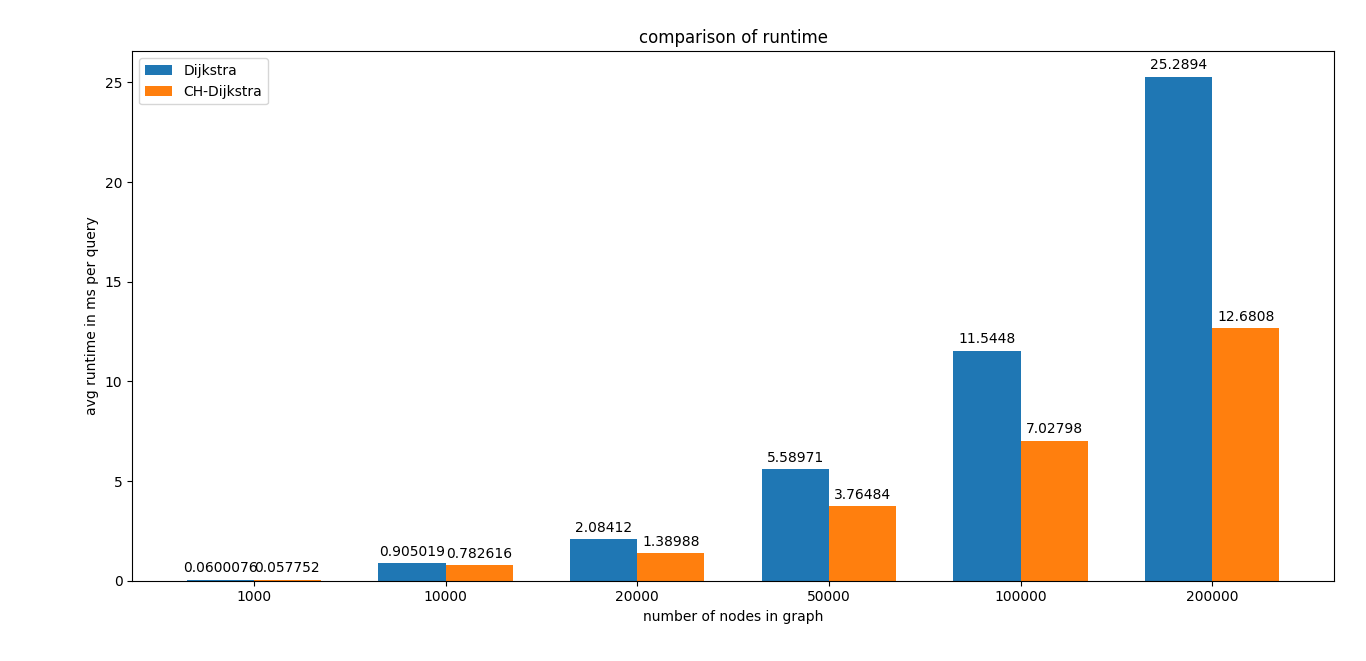
\includegraphics[width=0.9\textwidth]{benchmark-time.png}
  \vfill
\end{frame}
		
% ===================================================================================
\begin{frame}
  \thispagestyle{empty}
  \vspace{3cm}
  \begin{center}
	{\Huge \textbf{THE END}} \\
	{\large Thanks for listening!}
  \end{center}
\end{frame}
\end{huge}
		
\end{document}
